% =====================================================================
% CHAPTER 3 — RESULTS AND DISCUSSION
% =====================================================================
\chapter{Results and Discussion}
\label{ch:results}

\section{Baseline Results}
\label{sec:baseline}

The B0 baseline is strong for its cost: validation macro-F1 0.7093, test
macro-F1 0.7050 (MCC 0.4104, balanced accuracy 0.7047, bootstrap 95\% CI
$[0.6957, 0.7144]$). Training one seed takes 8.9 seconds and inference 0.50\,ms
per post. Its three seed runs are bit-identical (std $= 0.0000$), as expected for
a deterministic linear model---all seed variance in this study belongs to the
transformers, and the CI of the mean is correspondingly narrow. Two practical
readings follow: 0.7050 macro-F1 from a CPU model is a real bar that any
transformer must justify a GPU to beat, and the McNemar comparisons of
\S\ref{sec:significance} have a clean, noise-free reference.

\section{Main Comparison on the Test Set}
\label{sec:main}

Table~\ref{tab:main} reports the primary result: test macro-F1 as the 3-seed mean
$\pm$ standard deviation, the bootstrap 95\% CI around that mean, and the two
robustness metrics. Figure~\ref{fig:mainci} visualises the means with their CIs.

\begin{table}[htbp]
\centering
\caption[Main results on the PRISM test set]{Main results on the PRISM test set (3-seed mean $\pm$ std; CI is a
bootstrap 95\% interval around the mean, 1{,}000 resamples).}
\label{tab:main}
\small
\begin{tabular}{lrrrrr}
\toprule
Model & Macro-F1 & 95\% CI & MCC & Bal.\ acc. & Threshold \\
\midrule
B0 TF-IDF + SVM & 0.7050 $\pm$ 0.0000 & [0.6957, 0.7144] & 0.4104 & 0.7047 & --- \\
HingRoBERTa & 0.7300 $\pm$ 0.0046 & [0.7214, 0.7386] & 0.4639 & 0.7292 & 0.48 \\
MuRIL & 0.7254 $\pm$ 0.0036 & [0.7168, 0.7343] & 0.4582 & 0.7245 & 0.51 \\
XLM-RoBERTa & \textbf{0.7351 $\pm$ 0.0064} & [0.7265, 0.7439] & \textbf{0.4794} & \textbf{0.7344} & 0.51 \\
\bottomrule
\end{tabular}
\end{table}

\begin{figure}[htbp]
\centering
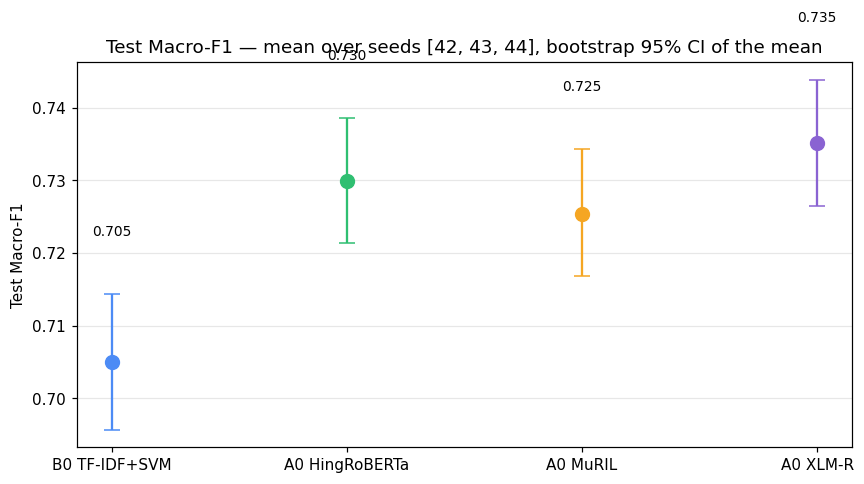
\includegraphics[width=0.66\textwidth]{figures/fig1_macro_f1_ci.png}
\caption[Test macro-F1: 3-seed mean with bootstrap 95\% CI]{Test macro-F1: 3-seed mean with bootstrap 95\% CI of the mean. The
transformer CIs sit above the baseline's, and largely above it outright.}
\label{fig:mainci}
\end{figure}

Three observations. First, \emph{pretraining wins, but modestly}: the best
transformer (XLM-R, 0.7351) beats the baseline by 0.0301 macro-F1, and the gap
between the best and worst transformer (0.0097) is smaller than the gap between
any transformer and the baseline. Second, \emph{the domain-matched model is not
the winner}: HingRoBERTa scores 0.7300, below the generalist XLM-R, though their
confidence intervals overlap heavily---the honest reading is ``XLM-R and
HingRoBERTa are statistically close; MuRIL trails both''. Third, \emph{seed noise
is real but small}: transformer stds (0.0036--0.0064) are an order of magnitude
below the baseline gap, so the ranking is not a one-seed accident---and
\S\ref{sec:significance} makes this precise.

\section{Per-Class Behaviour}
\label{sec:perclass}

Figure~\ref{fig:perclass} decomposes the headline numbers. The pattern is uniform
across all four models: the \emph{hate} class is the hard one. For XLM-R, hate
precision is actually the best in the table (0.762), but hate recall is the worst
cell (0.645)---the model misses roughly one hate post in three. Non-hate recall
for the transformers (0.79--0.82) exceeds hate recall by 13--18 points. The
baseline shows the same asymmetry in weaker form (hate recall 0.670).

Two consequences follow. First, the models are conservative: they prefer to label
an ambiguous post non-hate, which in a moderation pipeline means human review
queues absorb the misses. Second, because \emph{every} model shares this shape,
the cause is more likely in the data than in the architecture---boundary cases
where hateful intent is implied without explicit profanity are exactly the posts
that romanised, code-mixed text makes hardest to verify. This motivates the
threshold analysis in \S\ref{sec:threshold}: shifting the operating point trades
precision for recall directly.

\begin{figure}[htbp]
\centering
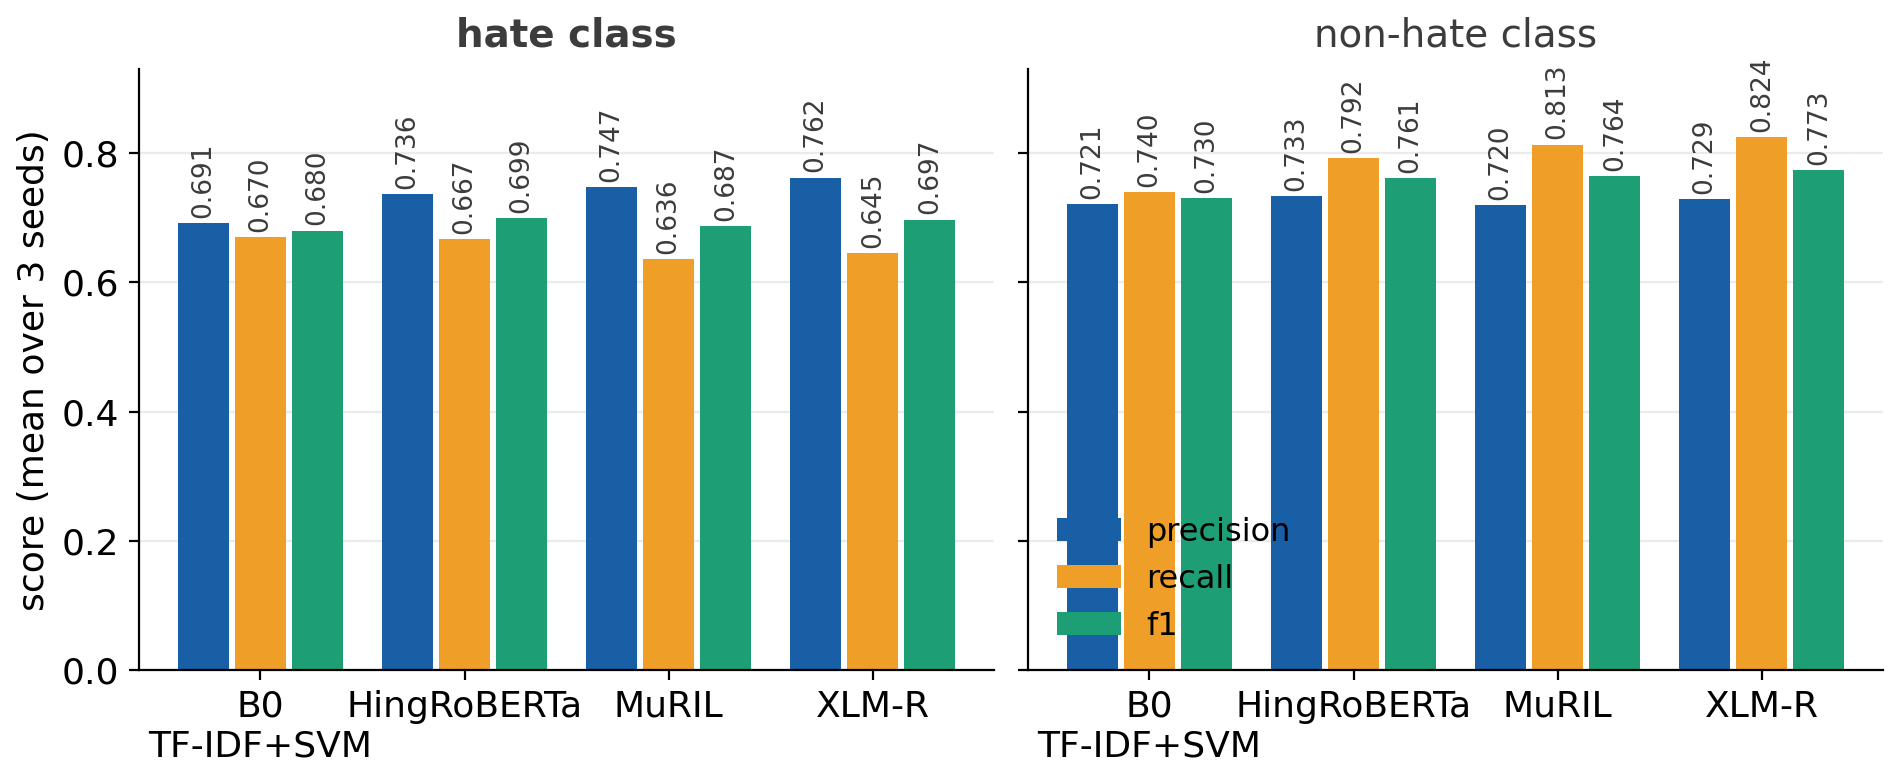
\includegraphics[width=0.98\textwidth]{figures/fig_per_class.png}
\caption[Per-class precision / recall / F1 on the test set]{Per-class precision / recall / F1 on the test set (mean over seeds).
Hate recall is the weakest cell for every model.}
\label{fig:perclass}
\end{figure}

\section{Statistical Significance}
\label{sec:significance}

Table~\ref{tab:mcnemar} reports the exact McNemar tests of each transformer
against B0 on the seed-42 test predictions, with Holm-corrected $p$-values across
the three comparisons. Every transformer wins: the discordant counts favour the
transformer in all three cases, and even the smallest margin (MuRIL: 1{,}094 vs.\
919 posts) is decisive after correction ($p_{\mathrm{adj}} = 3.1\times10^{-4}$).

\begin{table}[htbp]
\centering
\caption[Exact McNemar tests vs.\ B0 with Holm correction]{Exact McNemar tests vs.\ B0 (seed 42, $n = 8{,}852$). $n_{01}$: B0
correct, transformer wrong; $n_{10}$: transformer correct, B0 wrong. Holm
correction over the three comparisons.}
\label{tab:mcnemar}
\small
\begin{tabular}{lrrrl}
\toprule
Comparison & $n_{10}$ & $n_{01}$ & $p$ (exact) & $p$ (Holm-adj.) \\
\midrule
HingRoBERTa $>$ B0 & 1{,}263 & 980 & $2.5\times10^{-9}$ & $7.5\times10^{-9}$ \\
MuRIL $>$ B0 & 1{,}094 & 919 & $1.0\times10^{-4}$ & $3.1\times10^{-4}$ \\
XLM-R $>$ B0 & 1{,}181 & 841 & $4.1\times10^{-14}$ & $1.2\times10^{-13}$ \\
\bottomrule
\end{tabular}
\end{table}

Note what the test does and does not claim. It establishes that each transformer
is \emph{better than the baseline} on this test set, not that XLM-R is better than
HingRoBERTa---comparisons among the transformers were not tested, and given the
overlapping CIs of Table~\ref{tab:main} they would need more seeds to be
meaningful. The Holm correction is what licenses the word ``significant'' at all:
three uncorrected tests at $\alpha = 0.05$ would inflate the family-wise error
rate to about 14\%.

\section{Cost versus Quality}
\label{sec:cost}

Table~\ref{tab:costs} puts the accuracy table next to its price tag. Training a transformer seed takes 823--857 seconds against the
baseline's 8.9---a factor of about $96\times$ for XLM-R---and inference runs at
6.6\,ms per post against 0.50\,ms, a $13\times$ slowdown. The bought commodity is
$+0.0301$ macro-F1.

\begin{table}[htbp]
\centering
\caption[Cost of each model (mean over seeds)]{Cost of each model (mean over seeds). Training time excludes tokenisation
and data loading; inference is measured over the full test set.}
\label{tab:costs}
\small
\begin{tabular}{lrrr}
\toprule
Model & Params & Train time/seed & Inference \\
\midrule
B0 TF-IDF + SVM & --- & 8.9\,s & 0.50\,ms/post \\
HingRoBERTa & 278.0\,M & 856\,s & 6.56\,ms/post \\
MuRIL & 237.6\,M & 823\,s & 6.88\,ms/post \\
XLM-RoBERTa & 278.0\,M & 857\,s & 6.60\,ms/post \\
\bottomrule
\end{tabular}
\end{table}

Whether $96\times$ training and $13\times$ inference for three F1 points is a
good trade depends on the deployment. For a queue that screens millions of posts
the inference ratio alone is decisive: at 6.6\,ms per post one GPU core handles
$\sim$150 posts/s, the SVM $\sim$2{,}000 on CPU. A defensible hybrid reading is
to use the transformer where its three points matter most---the ambiguous middle
of the score distribution---and the SVM for the obvious remainder; this study
does not build that cascade, and lists it as future work (\S\ref{sec:future}).

\section{Training Behaviour and the Decision Threshold}
\label{sec:threshold}

The training dynamics are consistent across the transformers: training loss falls
steeply in the first epoch and validation macro-F1 rises with it, with most of the
achievable gain already present after the first of the three epochs. This explains
why the fixed three-epoch budget is not obviously under-provisioned for
fine-tuning, and it shows the plateau that the checkpoint policy (best validation
macro-F1) is designed to catch.

The validation macro-F1 surface over the swept threshold is flat near each
transformer's optimum---macro-F1 varies by less than half a point over a
$\pm$0.05 window---so the exact threshold is not a sensitive parameter. Table~\ref{tab:thresholds} makes the same point from the
other side: on the test set, the tuned threshold buys at most $+0.0022$ macro-F1
over the default argmax rule for XLM-R, and for MuRIL the tuned value is
marginally \emph{lower} than argmax. The value of the sweep is not the points it
buys but the bias it avoids: it removes ``0.5 was used by default'' as an
unexamined choice, and it moves one decision out of the test set.

\begin{table}[htbp]
\centering
\caption[Validation-tuned threshold vs.\ fixed 0.5 (seed 42)]{Validation-tuned threshold vs.\ fixed 0.5 (argmax) on the test set,
seed 42.}
\label{tab:thresholds}
\small
\begin{tabular}{lrrr}
\toprule
Model & Tuned thr. & Test F1 (tuned) & Test F1 (argmax) \\
\midrule
HingRoBERTa & 0.47 & 0.7363 & 0.7341 \\
MuRIL & 0.51 & 0.7206 & 0.7211 \\
XLM-RoBERTa & 0.53 & 0.7424 & 0.7408 \\
\bottomrule
\end{tabular}
\end{table}

\section{Error Analysis}
\label{sec:errors}

The error analysis uses the validation-selected backbone (XLM-R, seed 42) and
compares it to B0 throughout.

\subsection{Where the errors live: language and mixing level}
\label{sec:errors:lang}
Table~\ref{tab:perlang} splits the test set by post language. English posts are
the easiest for both models, and the transformer's advantage concentrates there
($+0.047$ macro-F1 over B0). Hindi and Hinglish posts are markedly harder; on
Hindi, the transformer's gain is nearly zero ($+0.002$). Since the test set
contains 2{,}900 Hindi and 1{,}407 Hinglish posts, a full third of the data
contributes almost none of the improvement.

\begin{table}[htbp]
\centering
\caption[Test macro-F1 by post language]{Test macro-F1 by post language (seed 42, $n$ = posts).}
\label{tab:perlang}
\small
\begin{tabular}{lrrr}
\toprule
Language & $n$ & B0 & A0 (XLM-R) \\
\midrule
English & 4{,}545 & 0.7723 & \textbf{0.8189} \\
Hindi & 2{,}900 & 0.6215 & 0.6233 \\
Hinglish & 1{,}407 & 0.6312 & 0.6680 \\
\bottomrule
\end{tabular}
\end{table}

Table~\ref{tab:buckets} re-cuts the same test set by the v2 mixing index. The
pattern is non-monotonic and initially surprising: the \emph{low-mixing} bucket is
the easiest (16.8\% error, macro-F1 0.8298), while the \emph{code-mixed} bucket
(0.2--0.5 minority share) is the hardest (32.0\% error, macro-F1 0.6274). Fully
monolingual posts are also hard (28.3\% error)---but for a different reason: that
bucket is dominated by short Hindi posts, the weakest language segment in
Table~\ref{tab:perlang}. The heavily mixed bucket ($\geq$0.5) is too small
($n = 72$) to support conclusions.

\begin{table}[htbp]
\centering
\caption[A0 errors by language-mixing bucket]{A0 (XLM-R) errors by language-mixing bucket on the test set (seed 42).}
\label{tab:buckets}
\small
\begin{tabular}{lrrrr}
\toprule
Bucket (mixing index) & $n$ & Error rate & Macro-F1 & Mean switches \\
\midrule
Monolingual ($<$0.05) & 5{,}070 & 0.2826 & 0.7170 & 0.4 \\
Low mixing (0.05--0.2) & 2{,}496 & \textbf{0.1679} & \textbf{0.8298} & 8.2 \\
Code-mixed (0.2--0.5) & 1{,}214 & \textbf{0.3196} & 0.6274 & 9.5 \\
Highly mixed ($\geq$0.5) & 72 & 0.1667 & 0.7000 & 7.9 \\
\bottomrule
\end{tabular}
\end{table}

\begin{figure}[htbp]
\centering
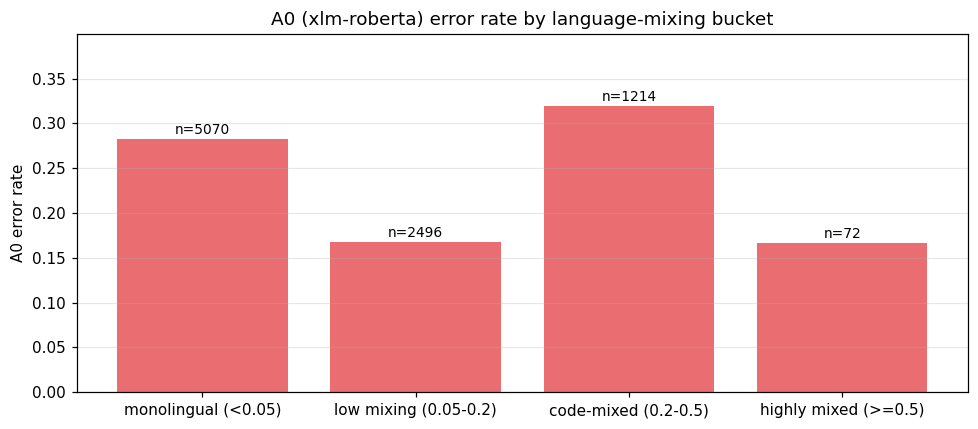
\includegraphics[width=0.62\textwidth]{figures/fig_error_phenomena.png}
\caption[A0 error rate by language-mixing bucket]{A0 (XLM-R) error rate by language-mixing bucket. The code-mixed bucket
is the peak of the error surface.}
\label{fig:errors}
\end{figure}

The reading is that \emph{true} code-switching---not romanisation alone, which
the subword vocabulary handles---remains the failure core of the task. A post
that alternates languages every few words (9.5 switches on average in the hard
bucket) requires the model to hold both languages' context in play, and neither
pretraining corpus taught it to do that at this frequency.

\subsection{Confusion structure}
Figure~\ref{fig:confusion} juxtaposes the two confusion matrices. The transformer
converts a large block of B0's non-hate errors into correct predictions (its
non-hate recall is 0.824 vs.\ 0.740) while its hate column looks similar to the
baseline's---consistent with \S\ref{sec:perclass}: the bought points are mostly
better \emph{non-hate} discrimination, i.e.\ fewer false accusations, while hate
recall barely moves (0.645 vs.\ 0.670).

\begin{figure}[htbp]
\centering
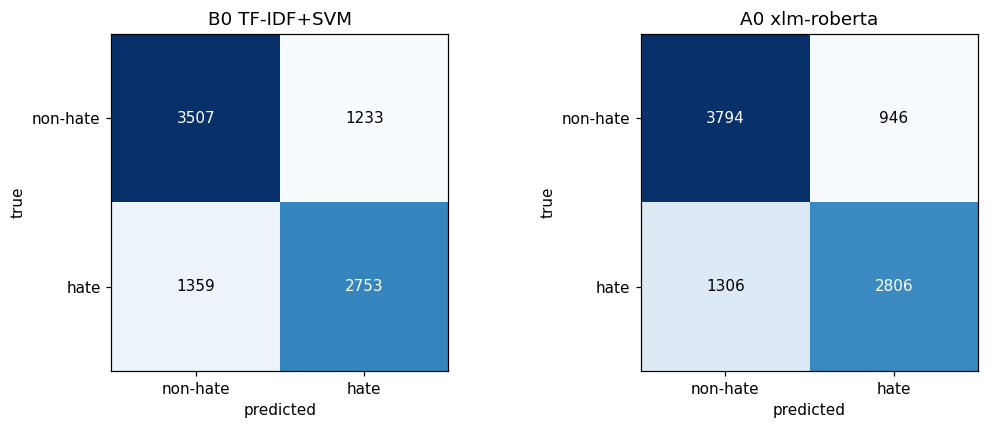
\includegraphics[width=0.72\textwidth]{figures/fig_confusion.png}
\caption[Confusion matrices: B0 vs.\ A0 (seed 42)]{Test-set confusion matrices (seed 42): B0 (left) vs.\ the
validation-selected A0 model (right).}
\label{fig:confusion}
\end{figure}

\subsection{Qualitative disagreements}
\label{sec:qualitative}
Table~\ref{tab:qualitative} shows posts on which B0 and A0 disagree, drawn from
the exported disagreement file (2{,}022 examples). The cases the transformer fixes
are long, sarcastic or implicit posts where lexical overlap misleads the linear
model; the cases it breaks are often short or borderline. Examples are shown in
Roman script; the export file also contains Devanagari rows.

\begin{table}[htbp]
\centering
\caption[Representative B0-vs-A0 disagreements]{Representative B0-vs-A0 disagreements (from 2{,}022 exported cases).
Posts are shown truncated; placeholders are the de-identification tokens of
\S\ref{sec:deid}.}
\label{tab:qualitative}
\scriptsize
\begin{tabular}{p{5.3cm}lccp{1.6cm}}
\toprule
Post (truncated) & True & B0 & A0 & Pattern \\
\midrule
``why are you making me jump through hoops when \ldots'' & 0 & 1 & 0 & A0 fixes false alarm \\
``laughing my ass off you guys i remember when s\ldots'' & 0 & 1 & 0 & A0 fixes false alarm \\
``are your friends safe living with a crush on y\ldots'' & 1 & 1 & 0 & A0 misses hate \\
``and you know he is probably saying the softest\ldots'' & 1 & 0 & 1 & A0 fixes miss \\
``give this up here is something you should take\ldots'' & 1 & 1 & 0 & A0 misses hate \\
\bottomrule
\end{tabular}
\end{table}

\section{Zero-Shot Cross-Lingual Transfer}
\label{sec:transfer}

Finally, the validation-selected model is applied, without any retraining, to the
416-post Marathi--English code-mixed test split of L3Cube-MeHate, carrying the
PRISM-validation threshold (0.53) unchanged. Table~\ref{tab:transfer} and
Figure~\ref{fig:transferfig} report the outcome: macro-F1 collapses from 0.7351
to 0.3770 (95\% CI $[0.3454, 0.4088]$)---a drop of 0.3581, and below the 0.5
level of a majority-vote classifier on this balanced set.

\begin{table}[htbp]
\centering
\caption[Zero-shot transfer from PRISM to MeHate]{Zero-shot transfer of the validation-selected A0 model (XLM-R, seed 42)
from PRISM (Hindi--English) to MeHate (Marathi--English), $n = 416$.}
\label{tab:transfer}
\small
\begin{tabular}{lrr}
\toprule
Setting & Macro-F1 & 95\% CI \\
\midrule
PRISM test (in-domain) & 0.7351 & [0.7265, 0.7439] \\
MeHate zero-shot (cross-lingual) & 0.3770 & [0.3454, 0.4088] \\
\midrule
Drop & 0.3581 & \\
\bottomrule
\end{tabular}
\end{table}

\begin{figure}[htbp]
\centering
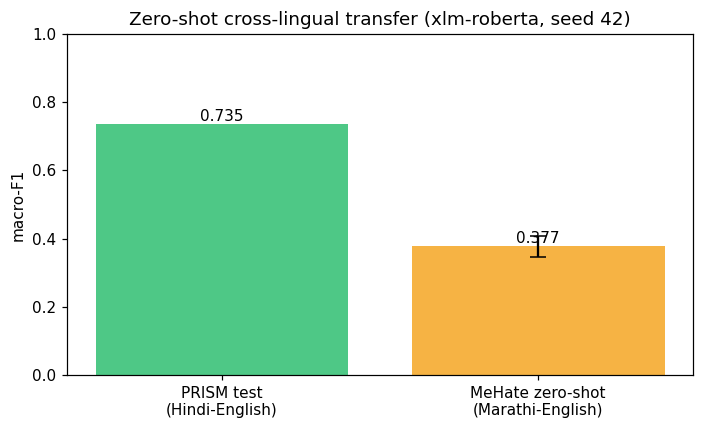
\includegraphics[width=0.48\textwidth]{figures/fig_transfer.png}
\caption[Zero-shot cross-lingual transfer]{Zero-shot cross-lingual transfer. The model that wins in-domain fails to
reach even chance-level behaviour out of domain.}
\label{fig:transferfig}
\end{figure}

Three confounds make the failure interpretable rather than merely embarrassing:
Marathi is (weakly) represented in XLM-R's pretraining but the fine-tuning
distribution is entirely Hindi--English; the MeHate split is small enough that
the CI is wide ($\pm$0.03); and the threshold was tuned for a different
probability calibration. Even granting all three, the conclusion stands: the
three-point in-domain advantage of pretraining does \emph{not} buy language
robustness for free. Transfer to a neighbouring Indian language fails, so the
idea of simply applying the PRISM model elsewhere is off the table, and
cross-lingual adaptation moves squarely into future work.

\section{Discussion}
\label{sec:discussion}

Returning to the problem statement: under an identical protocol, pretrained
multilingual encoders beat a character-level lexical baseline by about three
macro-F1 points on Hinglish hate-speech detection, the gain is significant under
Holm-corrected McNemar for every transformer, and the cost is roughly two orders
of magnitude in training time and one in inference latency.

The structure of the gain is as informative as its size. Pretraining bought
almost all of its improvement on English and lightly-mixed posts---the segments
where subword vocabulary robustness and world knowledge plausibly help---and
almost none on Devanagari Hindi or heavily code-switched posts, and none at all
out of domain. Domain-matched pretraining (HingRoBERTa) did not convert its
advantage into a win over the generalist, which suggests that at this data scale
the \emph{encoder capacity} matters more than the exact pretraining mixture, or
that 3 epochs of fine-tuning cannot re-align a domain-matched encoder better than
a strong general one. Both readings are consistent with the overlapping
confidence intervals and must be stated as hypotheses rather than findings.

The deployment-facing summary is threefold. First, the TF-IDF+SVM baseline is a
legitimate component, not a straw man: it costs seconds and reaches 0.7050. Any
report that compares transformers against nothing would overstate the value of
the GPU. Second, if the additional three points are needed, XLM-R is the
defensible choice, selected on validation, significant against the baseline. But
third---and this is the practical caveat---the added points concentrate on
non-hate recall, not on hate recall; the model that misses one hate post in three
gets only modestly less missed. For the actual goal of moderation, the hate
recall ceiling, not the leaderboard, is the frontier, and \S\ref{sec:future}
proposes the levers for it.
